\section{Physarum Polycephalum}
\label{section:background_physarum}

The organism being a subject for this work is \textit{Physarum Polycephalum} also called the many-headed slime mould. It is a member of the \textit{Physaridae} family of slime moulds, in order of \textit{Physarales}, class \textit{Myxogastria}, phylum \textit{Myxomycete}, supergroup \textit{Amoebozoa} in \textit{Protista} kingdom. While current position in taxology is well defined, presented characteristics will justify why scientists used to have problems with classification of the Physarum \cite{stephenson1994myxomycetes}.

In order to make the thesis readable, terms \textit{Physarum Polycephalum}, \textit{Physarum} or \textit{the slime mould} will be used interchangeably as the subject is unambiguously defined. As none of the authors have a background in biology, concepts are presented from a computer scientist's perspective in minimal, yet exhaustive, form.


\subsection{Biological characteristics}

\textit{Physarum Polycephalum} is a very peculiar organism. Even being a \textit{Protista} it can be observed with a naked eye --- it is a one amongst biggest living unicellular ogranisms \cite{TODO}. 

In its natural habitat, under cool, dark and humid conditions the slime mould exists in form of a yellow semistructurized blob (as seen in figure \ref{figure:bp_habitat}). Its occurrence is fairly common around the globe, however species \textit{Physarum Polycephalum} does not occur naturally in Poland \cite{narkiewicz2013grzyby}. It feeds on bacteria, fungi and other sources of basic nutrients.

In labaratory conditions, \textit{Physarum} is stored on Petri dishes filled with non-nutritious agar (figure \ref{figure:bp_petri}). The agar base provides humid environment required for supporting plasmodial stage of the slime mould. A sterille oats or even soft porridge is used as controlled source of nutrients. Complete description of storage and observation protocol, among other informations, is provided in Appendix \ref{chapter:protocol}.

\begin{figure}
  \centering
  % TODO find another image
  \begin{subfigure}{0.45\textwidth}
    \centering
    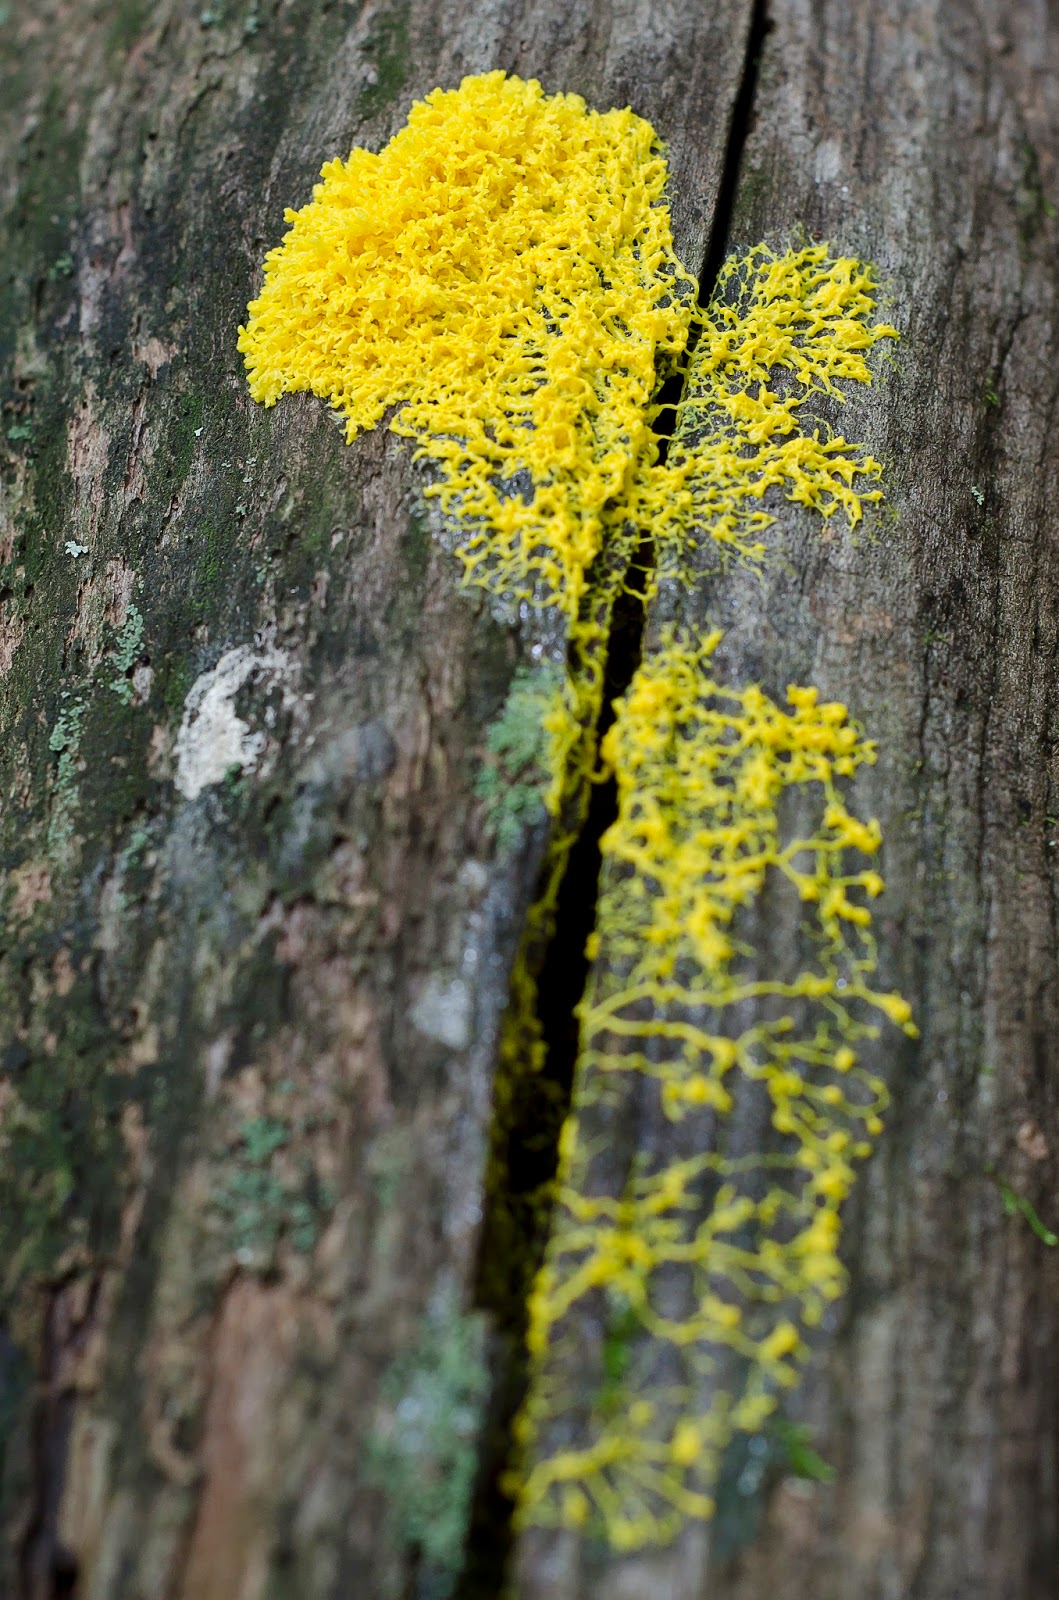
\includegraphics[width=0.44\textwidth]{background/physarum/habitat.jpg}
    \caption{Natural habitat \cite{TODO}}
    \label{figure:bp_habitat}
  \end{subfigure}
  \begin{subfigure}{0.45\textwidth}
    \centering
    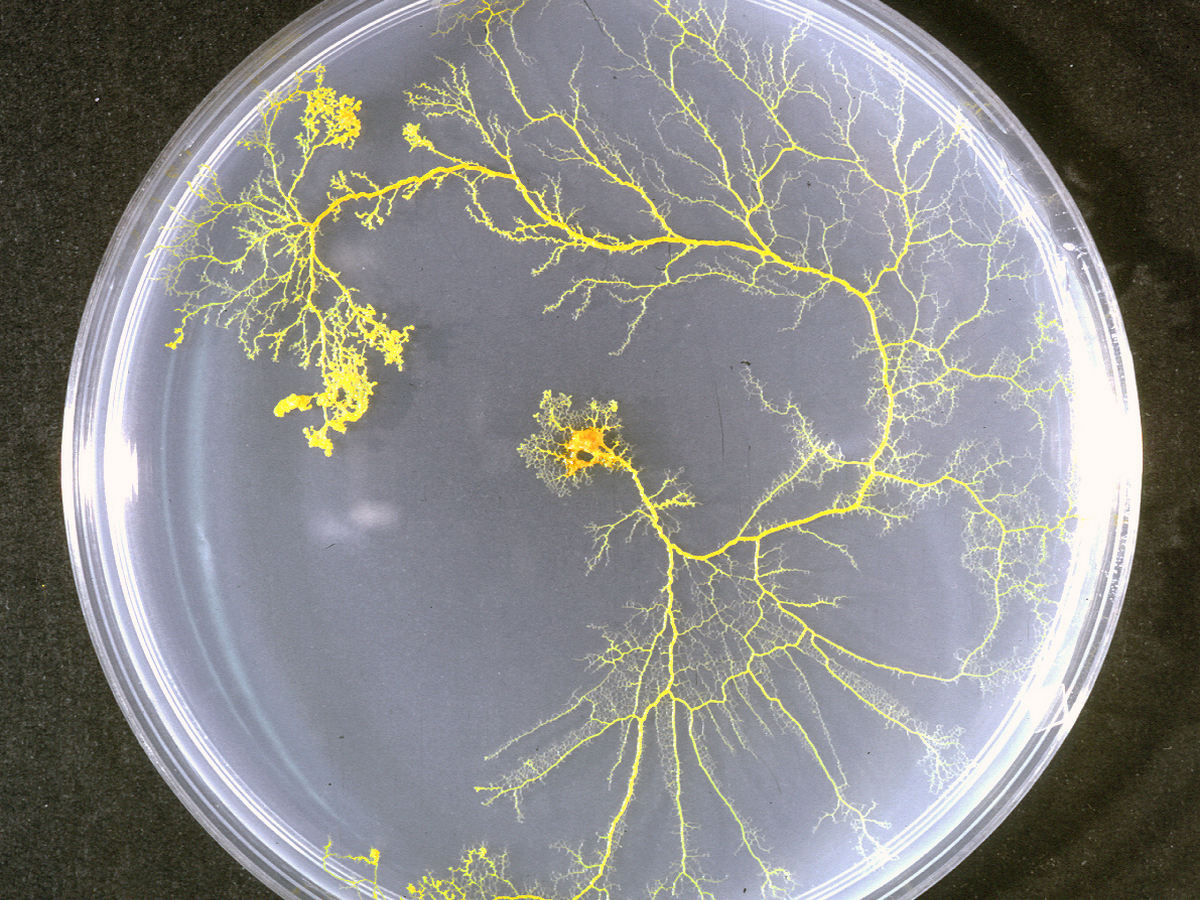
\includegraphics[width=0.9\textwidth]{background/physarum/petri.jpg}
    \caption{Petri dish}
    \label{figure:bp_petri}
  \end{subfigure}
  \caption{\textit{Physarum Polycephalum} in plasodial stage}
\end{figure}

% TODO preferred image from carolina
\begin{figure}
  \centering
  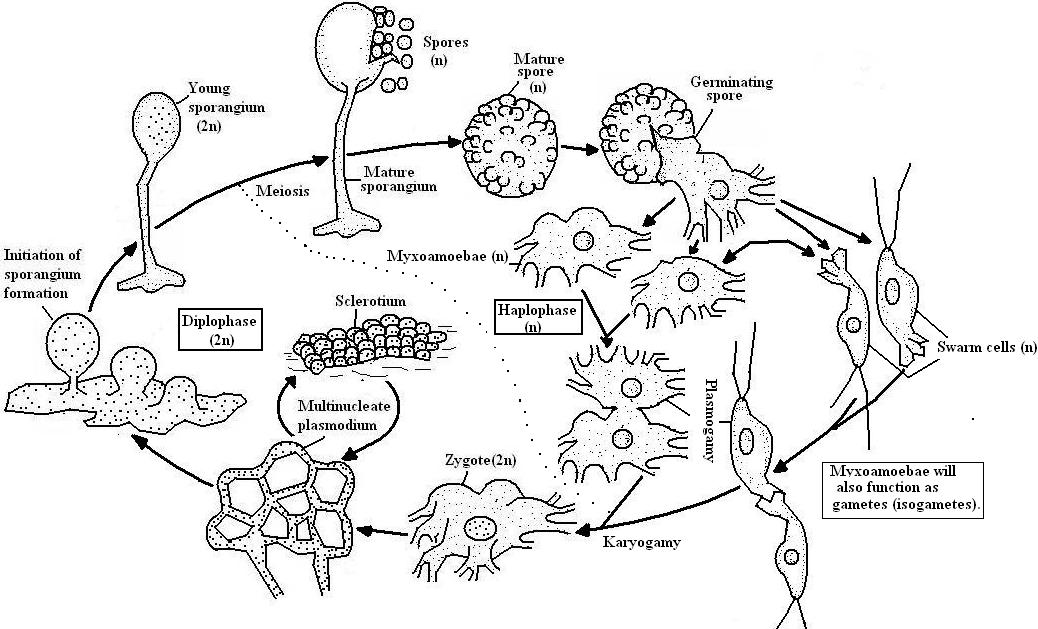
\includegraphics[width=0.94\textwidth]{background/physarum/lifecycle.png}
  \caption{Lifecycle of \textit{Physarum Polycephalum} \cite{TODO}}
  \label{figure:bp_lifecycle}
\end{figure}

As representant of \textit{Myxomycete}, a life cycle of the slime mould is very complex including haploid and diploid phases (as seen in figure \ref{figure:bp_lifecycle}). Such cycle is result of evolutionary adaptation. Formation of sporangium occurs in result of worsening conditions (such as inadequate temperature, humidity or acidity). Sporangium releases spores, which can germinate into ameboid swarm cell. Such cell can enclose itself into a cyst to protect the cells until environmental conditions improve. When conditions are favourable amoeboid cell turns into flagellated swarm cell. Swarm cells can merge, fuse their nuclei and start mitotic process resulting in forming a plasmodium \cite{jones2015pattern}.

For purposes of unconventional computing applications, \textit{Physarum} is preferred in its such plasmodial stage. However, during research transformations into other states are inevitable and must be dealt with. In case of drying and enforced starvation sclerotium is formed --- in this dormant phase \textit{Physarum Polycephalum} can survive for many years until dampness and nutrients are provided again.

Plasmodium forms protoplasmic tubes (also called pseudopodia) accordingly to food availability. Such tubes are used for discovery and transportation of nutrients. The tubes are built in similar way to animal muscles. The ectoplasm contains actin and myosin complexes, which are organised into regular structures forming tubes. Such actomyosin complexes generate contractile motion resulting in streaming of protoplasm. Furthermore, synchronized oscillations of protoplasm stream direction can observed. Nutrients are transported in one direction, after 1-2~minutes the direction is reversed. Period of this oscillation depends on environment quality and accesibility to food \cite{wohlfarth1979oscillatory} --- higher frequency oscillations are generated where nutrients available and no harmful environment exist, low frequency oscillations are caused by lack of food or as a result of unfavourable conditions. 

The plasmodium can grow around 10~mm per hour when actively exploring environment \cite{coggin1996dynamic}. While moving, plasmodium leaves polysaccharide traces (informally called slime, hence the name slime mould). Network of the protoplasmic tubes adapts, forming efficient ways of transporting nutrients, depending on their amount and quality \cite{nakagaki2004obtaining}. Usage of this behaviour is a fundamental principle for building physarum machines.


\subsection{Related works}

Since early 1960s \textit{Physarum Polycephalum} has been a subject to many biological and microbiological studies \cite{guttes1964mitotic,daniel1962method}, however it is late 70s when its computational-like behaviours have been observed \cite{wohlfarth1979oscillatory}.

% TODO artists
Research towards computational applications of the \textit{Physarum} truly started in 1990s. Nowadays, there exist two prominent research centers focusing on the slime mould --- one based in United Kingdom (Andrew Adamatzky\footnote{~\url{http://uncomp.uwe.ac.uk/adamatzky/}}, Jeff Jones\footnote{~\url{http://uncomp.uwe.ac.uk/jeff/}} from University of West England, Bristol), other one in Japan (Toshiyuki Nakagaki\footnote{~\url{http://www.cris.hokudai.ac.jp/cris/en/research/ob/ob\_innovative/nakagaki.html}}, Hokkaido University, Sapporo). Some of their works excited us about slime mould capabilities and inspired to write this thesis \cite{nakagaki2000intelligence,adamatzky2010physarum,jones2015pattern,adamatzky2007physarum}. Experiments presented here, focus on different aspects of \textit{Physarums} behaviour. Analyzing and understanding them gives impression of emerging computational power of such simple organism as a slime mould.


\subsubsection{Maze-solving capabilities}

Maze-solving or more constricted problem of finding, preferably shortest, paths is very common in practice. It has many applications and many possible algorithms are already available. Algorithms such as breadth-first search or more complex $A*$ are commonly used for solving mazes \cite{zelkowitz1979principles}, however Toshiyuki Nakagaki et al. proposed usage slime moulds' natural capabilities as unconventional solution to this problem \cite{nakagaki2000intelligence}.

In order to use \textit{Physarum} to solve a labiryth, a maze must be represented as a physical object. Such maze is modelled on a Petri dish where floor is made of non-nutrient agar and walls are made of thin plastic film (the maze used in the experiment is presented on figure \ref{figure:bp_maze_initial}). As the slime mould strictly prefers humid environment of the agar it will not pass arid walls made of plastic film. 

\begin{figure}
  \centering
  \begin{subfigure}{0.45\textwidth}
    \centering
    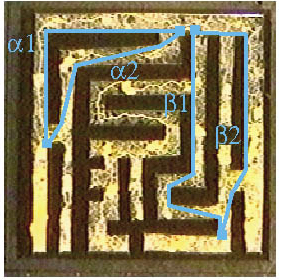
\includegraphics[width=0.9\textwidth]{background/physarum/maze1.jpg}
    \caption{Plasmodium initially filling maze}
    \label{figure:bp_maze_initial}
  \end{subfigure}
  \begin{subfigure}{0.45\textwidth}
    \centering
    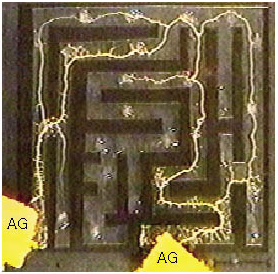
\includegraphics[width=0.9\textwidth]{background/physarum/maze2.jpg}
    \caption{Intermediate state}
    \label{figure:bp_maze_intermediate}
  \end{subfigure}
  \begin{subfigure}{0.45\textwidth}
    \centering
    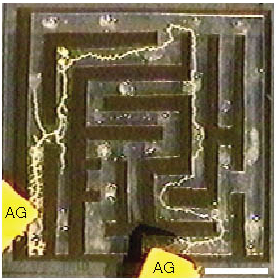
\includegraphics[width=0.9\textwidth]{background/physarum/maze3.jpg}
    \caption{Final route}
    \label{figure:bp_maze_final}
  \end{subfigure}
  \caption{\textit{Physarum} in various states of the maze experiment \cite{nakagaki2000intelligence}}
\end{figure}

There are four possible routes available $\{(\alpha_1,\beta_1), (\alpha_1,\beta_2), (\alpha_2,\beta_1), (\alpha_2,\beta_2)\}$ between entry point $A$ and exit point $B$. Oatmeal-agar based source of nutrients is planted in both entry and exit points, while large enough plasmodium is placed over whole floor of the maze. As time passes it can be observed that plasmodium retracts its body from labirth's dead-ends, leaving traces of slime where it previously has been placed (figure \ref{figure:bp_maze_intermediate}). 

As a result the slime mould rests only on direct paths connecting an entry with an exit point (figure \ref{figure:bp_maze_final}). Furthermore, it has been observed that \textit{Physarum Polycephalum} usually prefers shortest $(\alpha_2,\beta_1)$ path as it prefers most efficient way for transferring nutrients. While obtained results are satisfactory, it must be noted that whole process takes about 4~hours. 


\subsubsection{Spatial memory}

Memory is usually associated with neurological functions of brain, however it can be externalized in multiple ways, in example as pheromone trails of ants \cite{carroll1973ecology} or even notes-writing as humans do \cite{fisher1973effect}. Team of researchers from University of Sydney, demonstrated that \textit{Physarum Polycephalum} uses its slime as a form of spatial externalized memory \cite{reid2012slime}.

A common problem testing autonomous navigational skills in robotics is U-shaped trap problem \cite{chatterjee2001use}. Efficient solution of the issue requires some kind spatial memory or other navigational aids \cite{balch1993avoiding}, therefore it was a good candidate for a test of slime mould's memoizing capabilities. U-maze problem requires an agent (a robot or as in this example the slime mould) to navigate itself from starting position to the goal, where goal is hidden beside an u-shaped trap (figure \ref{figure:bp_trap_model}). The agent has to use some kind of environment map or use reactive guidance to bypass the trap (figure \ref{figure:bp_trap_model_success}), otherwise, most probably, it will be stuck inside the trap (figure \ref{figure:bp_trap_model_failure}).

% TODO create vector images like these
\begin{figure}
  \centering
  \begin{subfigure}{0.45\textwidth}
    \centering
    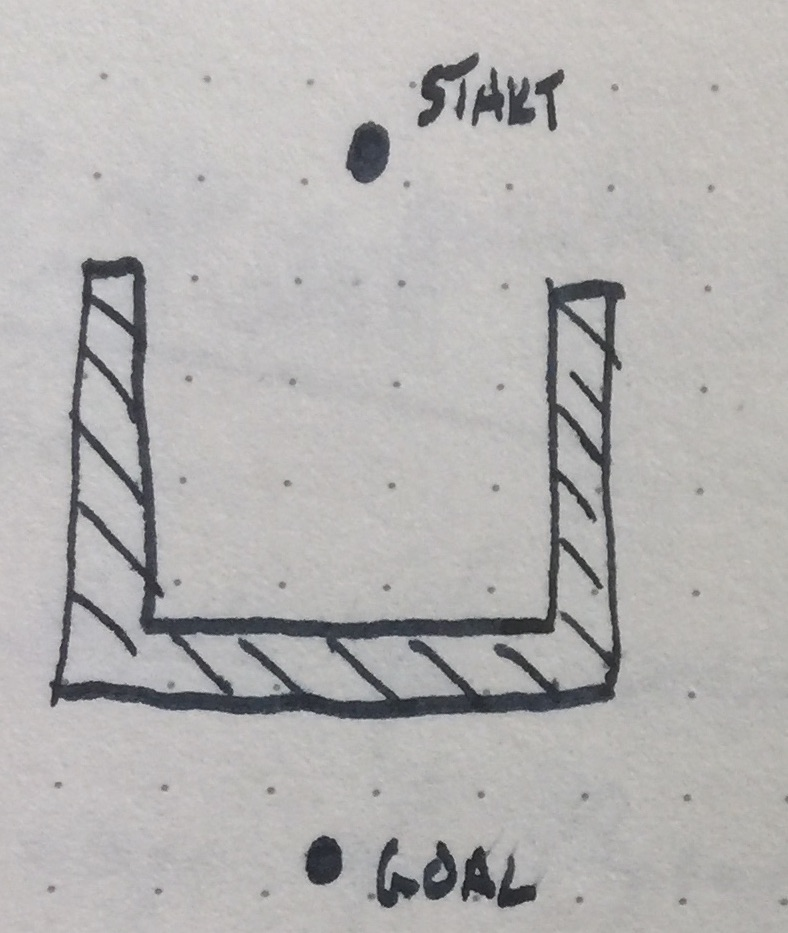
\includegraphics[width=0.9\textwidth]{background/physarum/trap_model_initial.jpg}
    \caption{Initial setup}
    \label{figure:bp_trap_model}
  \end{subfigure}
  \begin{subfigure}{0.45\textwidth}
    \centering
    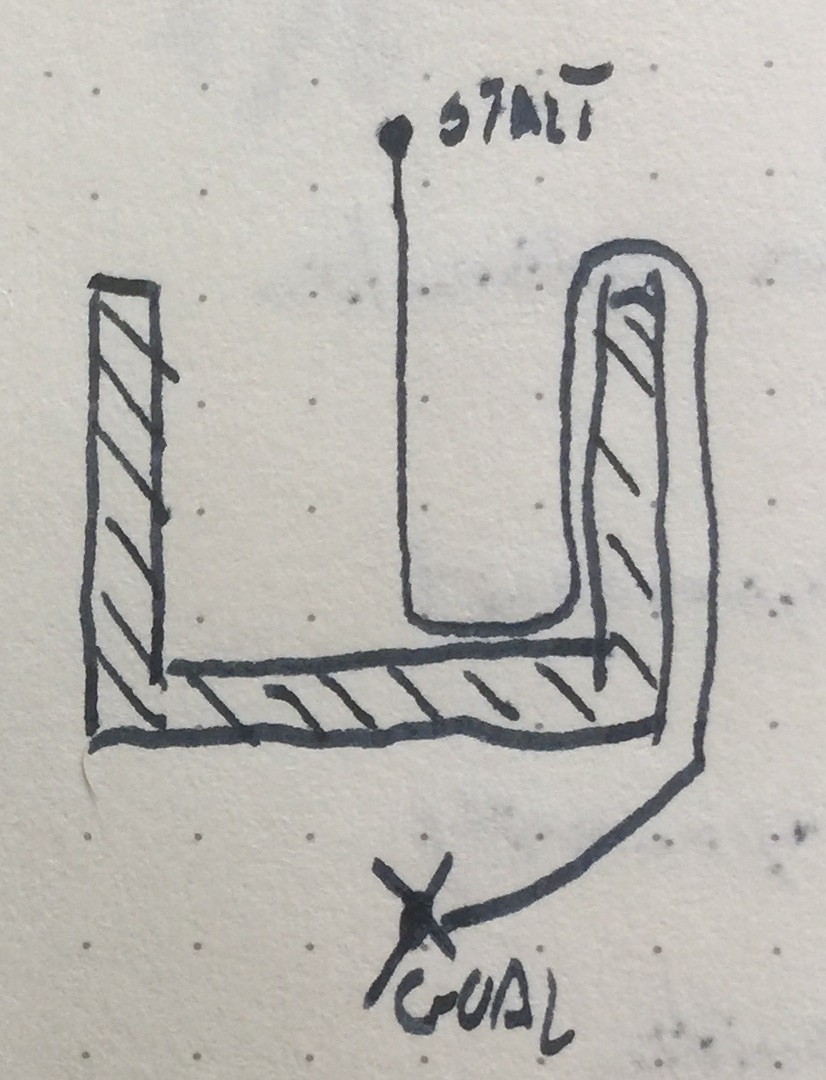
\includegraphics[width=0.9\textwidth]{background/physarum/trap_model_success.jpg}
    \caption{Example successful route to goal}
    \label{figure:bp_trap_model_success}
  \end{subfigure}
  \begin{subfigure}{0.45\textwidth}
    \centering
    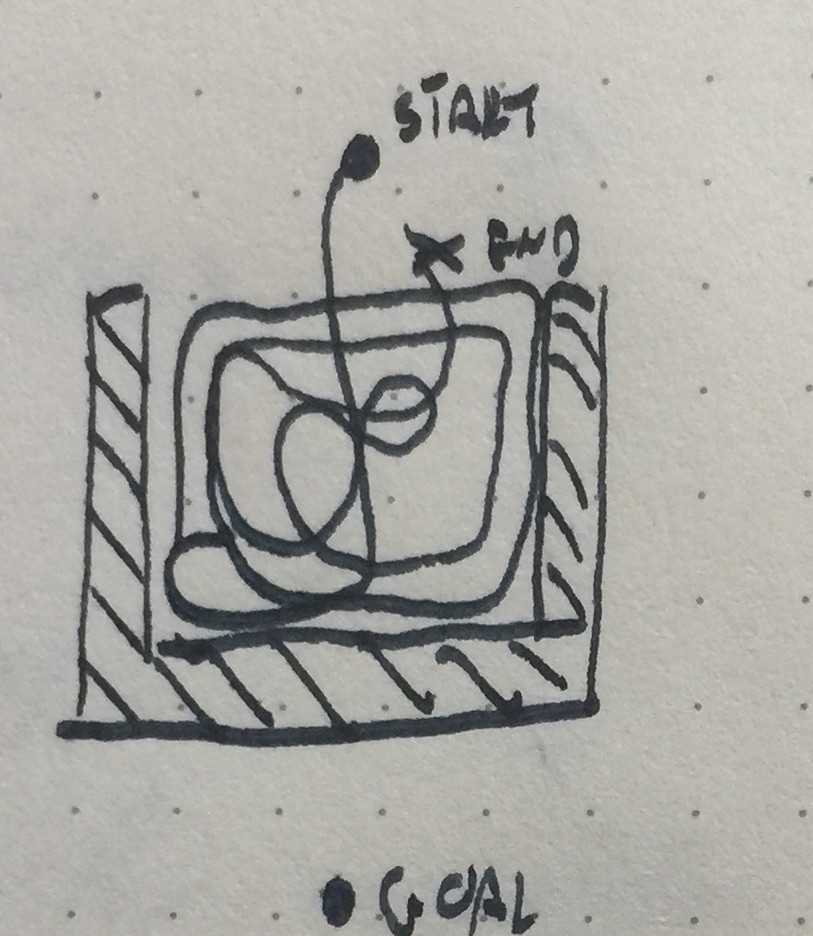
\includegraphics[width=0.9\textwidth]{background/physarum/trap_model_failure.jpg}
    \caption{Typical failure}
    \label{figure:bp_trap_model_failure}
  \end{subfigure}
  \caption{U-trap test with possible outcomes}
\end{figure}

The experiment conducted by Reid, Latty, Dussutour and Beekman \cite{reid2012slime} used \textit{Physarum Polycephalum} as an agent in non-nutrient agar environment, where the trap was made out of acetate and the goal was highly nutritious glucose. Agar base allows diffusion of glucose particles, resulting in nutrients gradient towards the goal.

Initial experiments indicated that \textit{Physarum} moves in direction where its slime is not present, however if no such direction exists (that is there is the slime all around plasmodium) it moves in random direction or all over the substrate. Therefore a slime mould has a choice to explore unexplored, however it is not an ultimate one, as it always can maneuver in previously visited areas. 

\begin{figure}
  \centering
  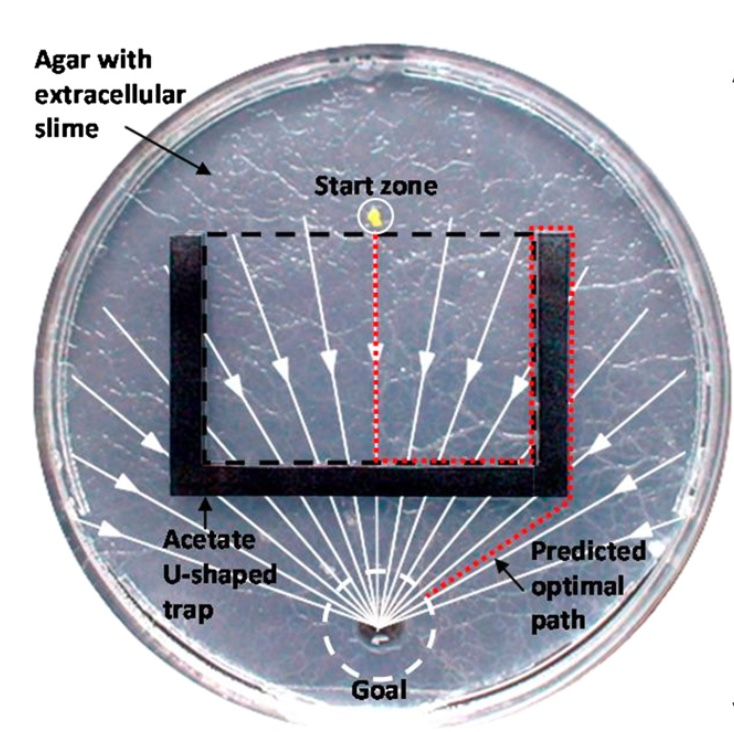
\includegraphics[width=0.74\textwidth]{background/physarum/trap_experiment.jpg}
  \caption{\textit{Physarum Polycephalum} in U-trap experiment on a slime covered substrate \cite{reid2012slime}}
  \label{figure:bp_trap_experiment}
\end{figure}

As the slime is stable, nonliving substance mostly made of galactose polymers it can be easily handled, collected and replanted \cite{mccormick1970isolation}. Two varieties of the experiment has been designed --- in a first one, previously collected slime is placed all over the substrate (figure \ref{figure:bp_trap_experiment}), where in a second one the substrate is just a clean agar. The first environment constrains \textit{Physarum} not to rely on slime for navigation (as provided slime acts as noise), unlike the second one, in which \textit{Physarum} can use the slime freely for its navigation.

Experiments have shown that \textit{Physarum} placed on a substrate already coated with the slime cannot easily escape out of the U-trap --- it spends there a long time until it leaves the trap. Furthemore, only in 33\% of 24 repeated cases plasmodium reaches the goal. However, when plasmodium is put on a clean agar substrate, an ability to use its slime as navigational aid results in reaching the goal in 96\% of cases. Both travelled distance and time to reach the goal were much shorter when the organism were able to use the slime. These findings prove that \textit{Physarum Polycephalum} can sense its extracellular slime and uses its existence as form of externalized spatial memory for recognition of previously explored areas.


\subsubsection{Adaptive network design}

lorem tokyo


\subsection{Observations}

lorem


\subsubsection{Sensoric input}

% nasa gravisens
lorem


\subsection{Computer models}

lorem


